\chapter{Title} % Main chapter title
\label{chap:ChapterX}  % For referencing this chapter elsewhere, use \ref{Chapter1}
\epigraph{``” }{\textit{}}

% 
% Single Figure
% 
\begin{figure} [H]
	\centering
	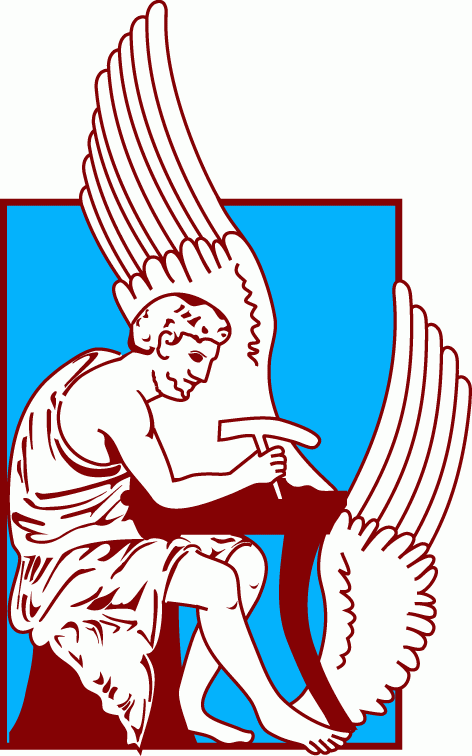
\includegraphics[scale=0.3]{Images/TUC_logo.png}
	\decoRule
	\caption[UAV]{\hyperref[abbr:UAV Sample]{UAV Sample}: \href{google.com}{URL}}
	\label{fig:UAV-sample}
\end{figure}

% 
% Side by side two Figures
% 
\begin{figure} [H]
    \centering
    % -----------------
    \begin{minipage}{.5\textwidth}
      \centering
      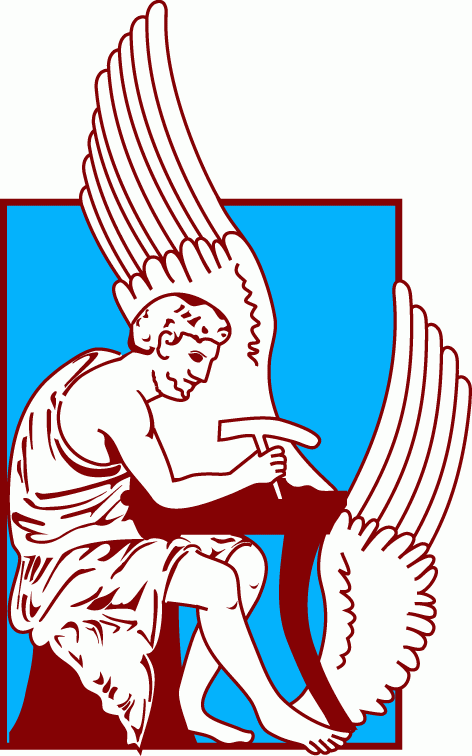
\includegraphics[width=.4\linewidth]{Images/TUC_logo.png}
      \decoRule
      \caption[UAV]{\hyperref[abbr:UAV Sample]{UAV Sample}: \href{google.com}{URL}}
      \label{fig:UAV-sample1}
    \end{minipage}%
    % -----------------
    \begin{minipage}{.5\textwidth}
      \centering
      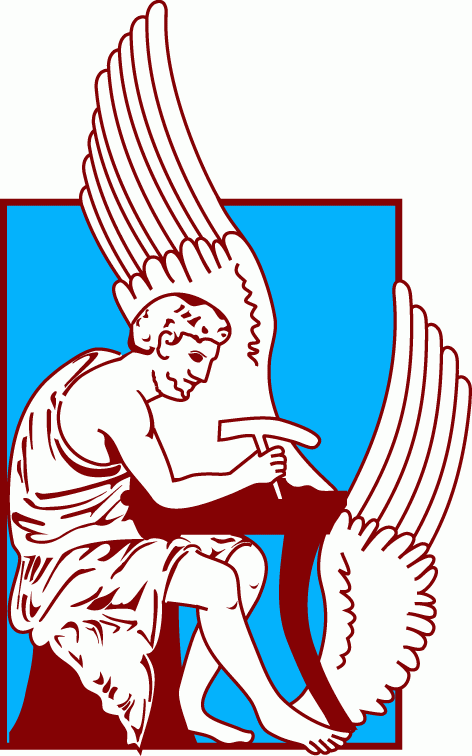
\includegraphics[width=.4\linewidth]{Images/TUC_logo.png}
      \decoRule
      \caption[UAV]{\hyperref[abbr:UAV Sample]{UAV Sample}: \href{google.com}{URL}}
      \label{fig:UAV-sample2}
    \end{minipage}
    % -----------------
\end{figure}

% 
% Table
% 
\begin{table}[H]
    \caption{}
    \label{tab:}
    \centering
    \begin{tabular}{llll}
        \toprule
        \textbf{Layer} & \textbf{\#Parameters} & \textbf{Footprint} & \textbf{Memory (\%)}  \\
        \midrule
            Conv1 & $64 * 3 * 11 * 11 = 23232$ & 92.92KB & 0.04 \\
        \midrule
            \textbf{Total} & 61090496 & 244.36MB & 100 \\
        \bottomrule
    \end{tabular}
\end{table}


\begin{align}
	\mathcal{E}[Y(t+\tau)Y(t)] = R_{yy}(t+\tau,t) =& \mathcal{E} [X( t + \tau) \cos(2 \pi f_0 (t + \tau) + \Theta) X(t) \cos(2 \pi f_0 t + \Theta)] \nonumber \\
	\overset{indep.}{=}& \mathcal{E}[X(t+\tau)X(t)] \mathcal{E}[\cos(2\pi f_0(t+\tau) +\Theta)\cos(2\pi f_0t + \Theta)] \nonumber \\
	\overset{(\ref{cosa-cosb})}{=}& \mathcal{E}[X(t+\tau)X(t)]\frac{1}{2}\mathcal{E}[\cancelto{0}{\cos(4\pi f_0t+2\pi f_0\tau+2\Theta)} + \cos(2\pi f_0\tau)] \nonumber \\
	=& \frac{1}{2} \mathcal{E}[X(t+\tau)X(t)] \cos(2\pi f_0\tau) \nonumber \\ 
	=& \boxed{ \frac{1}{2} R_{xx}(t+\tau,t)\cos(2\pi f_0\tau)}
\end{align}


%
% Algorithm
% 

\begin{algorithm}[H]
	\caption{Convolution Layer}\label{alg:Convolution-Layer}
	\begin{algorithmic}[1]
		\Procedure{Convolution Layer}{input, kernelSize, stride, padding, weights, bias}
			\State $hOut \gets (input.height +2 * padding - kernelSize) / stride + 1$
			\State $wOut \gets (input.width +2 * padding - kernelSize) / stride + 1$

			\For{i:=1 \textbf{to} input.channels}
				\For{j:=1 \textbf{to} input.height + 2 * padding}
					\For{k:=1 \textbf{to} input.width + 2 * padding}
						\If{j <= padding || k <= padding || j > image.height + padding || k > image.width + padding}
							\State $arr(i, j, k) \gets 0$
						\Else{}
							\State $arr(i, j, k) \gets input(i, j - padding, k - padding)$
						\EndIf
					\EndFor
				\EndFor
			\EndFor

			\For{oc:=1 \textbf{to} size(weights, 1)} \Comment{\#Output channels}
				\For{oh:=1 \textbf{to} hOut}
					\State $imgStartH \gets oh * stride$
					\State $imgEndH \gets imgStartH + kernelSize$

					\For{ow:=1 \textbf{to} wOut}
						\State $imgStartW \gets ow * stride$
						\State $imgEndW \gets imgStartW + kernelSize$

						\State $pixel \gets 0$
						\For{ic:=1 \textbf{to} input.channels}
							\For{i:=1 \textbf{to} kernelSize}
								\For{j:=1 \textbf{to} kernelSize}
									\State $pixel \gets pixel + arr(ic, i + imgStartH, j + imgStartW) * weights(oc, ic, i, j)$
								\EndFor
							\EndFor
						\EndFor

						\State $output(oc, oh, ow) \gets pixel + bias(oc)$
					\EndFor
				\EndFor
			\EndFor
			\State \textbf{return} $output$
		\EndProcedure
	\end{algorithmic}
\end{algorithm}